\documentclass{beamer}

%\usepackage{graphicx}
%\usepackage{tikz}
%\usepackage[absolute,overlay]{textpos}
%\usepackage{listings}
%\usepackage{textpos}
\usepackage{graphicx}


%\includeonlyframes{1,2,3}


\usetheme{Antibes}
% Orange
\usecolortheme[RGB={32,115,53}]{structure}

\usebackgroundtemplate{
    % UniCT Logo
    
\includegraphics[width=370pt]{img/unict.jpg}
}

\newtheorem{samplecode}{Sample Code}

%\setbeamercovered{transparent}
\setbeamertemplate{footline}[frame number]{}
\setbeamertemplate{blocks}[rounded][bg=red]

\newcommand{\tildett}{\raise.17ex\hbox{$\scriptstyle\mathtt{\sim}$}}
% Spaces
\newcommand{\N}{\vskip 0.3 cm}
\newcommand{\n}{\vskip 0.2 cm}
\newcommand{\TAB}{\hskip 1.8 cm}
\newcommand{\tab}{\hskip 0.6 cm}

% Colors
\newcommand{\red}[1]{\textcolor[rgb]{.8,0,0}{#1}}
\newcommand{\blue}[1]{\textcolor[rgb]{0,0,.7}{#1}}
\newcommand{\navy}[1]{\textcolor[rgb]{0,0,.5}{#1}}
\newcommand{\purple}[1]{\textcolor[rgb]{.7,0,.8}{#1}}
\newcommand{\green}[1]{\textcolor[rgb]{0,.6,.1}{#1}}


\title[Un sistema per il monitoraggio di impianti fotovoltaici]{
  Un sistema per il monitoraggio di \\ impianti fotovoltaici
 }\subtitle[]{Progetto e implementazione}
\author{Loris Fichera \n
Relatore: Prof. Corrado Santoro}
\institute[Universit\`a di Catania]{
	Universit\`a degli Studi di Catania\\
        Corso di Laurea Specialistica in Ingegneria Informatica\\
}
\date{20 Luglio 2011}


\begin{document}

% Title Page
\begin{frame}[plain]
  \titlepage
\end{frame}
%

%% \begin{frame}
%% \tableofcontents
%% \end{frame}

%------------------------------
%% \begin{frame}[shrinks,label=o]{Outline}
%% %  \tableofcontents[pausesections]
%% %     \tableofcontents
%%     \begin{columns}
%%      \column{2.0in}
%% %       \tableofcontents[sections={1}]
%% %      \vspace{10mm}
%%        \tableofcontents[sections={2}]
%%       \vspace{10mm}
%%        \tableofcontents[sections={3}]
%%        \column{2.0in}
%%        \tableofcontents[sections={4}] 
%%        \vspace{10mm}
%%       \tableofcontents[sections={5}] 
%% %      \vspace{10mm}
%% %       \tableofcontents[sections={5}]
%%       \end{columns}
%% \end{frame}
%------------------------------

\section{Introduzione}
\begin{frame}{Monitoraggi \emph{immaturi}}
  Il numero di impianti fotovoltaici \emph{grid-connected}, in Italia, \`e in costante aumento
  \begin{itemize}
    \item potenza installata \red{raddoppia} ogni anno
    \item oltre \red{4 GW} al 31/12/2010
  \end{itemize}
  \N
  Il problema del monitoraggio assume importanza per 
  \begin{itemize}
    \item i \green{soggetti responsabili}
    \item gli \green{installatori/manutentori}
  \end{itemize}
  \N
  "Gran parte delle soluzioni oggi in commercio mostrano caratteri di \emph{immaturit\`a}" (C. Podewils 2010)
\end{frame}
%

%
\section{Il monitoraggio di impianti fotovoltaici}
\subsection{Definizione del Problema}
\begin{frame}{Obiettivi}
Un sistema di monitoraggio effettua la \green{raccolta} e \green{l'integrazione} dei dati \red{rilevanti} di un impianto al fine di
determinarne:
%
\begin{itemize}
\item lo stato operativo
\item l'efficienza globale
\item la produzione energetica
\end{itemize}
%
\begin{figure}[!h]
  \begin{center}
    \fbox{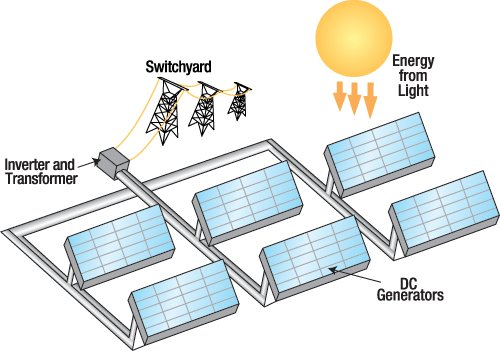
\includegraphics[width=170pt]{img/solar_photovoltaic.jpg}}
  \end{center}
\end{figure}
%
\end{frame}
%












%%\section*{Introduction}

%\subsection{}
%
%\begin{frame}{Problem Statement}  
%  \begin{itemize}
%    \item Our work aims at \ldots
%    \item More\dots
%  \end{itemize}
%  \vfill
%  A whitespace gap\\
%  \begin{tiny}
%    Smaller Font
%  \end{tiny}
%\end{frame}
%%


%----------------------------- Core concepts of PROFETA
%% \section{Profeta}

\subsection{Motivation}
%------------------------------
\begin{frame}[label=1]{AMR Programming}
  %
  \begin{itemize}
    \item
      The software running on \red{A}utonomous \red{M}obile \red{R}obots
      requires the execution of many different tasks
\N  
    \item
      \red{Low level} tasks are typically written in imperative languages 
        %(\purple{C}, \purple{assembly})
\n
    \item
      \red{Higher level} tasks, e.g. strategy control, could benefit 
      from a logic/declarative approach
\N\N  
\pause
    \item
      \navy{Profeta} embeds declarative constructs into Python by
      using the BDI model and exploiting operators overloading
\n    
    \item
      \navy{Profeta} provides an all-in-one environment, while combining
      the advantages of both approaches
%      into an imperative language, to provide an all-in-one environment
%    \item A combination of both paradigms seems a reasonable trade-off
  %
  \end{itemize}
% 
\N\N
\end{frame}
%------------------------------



\subsection{The BDI Model}
%------------------------------
\begin{frame}[label=2]{The Belief-Desire-Intention Model}
  %
  \begin{itemize}
    \item
      The BDI model is a philosophical theory of human reasoning 
      %[\purple{Bratman et Israel}] 
      that has been successfully applied to \red{software agents} 
      %[\purple{Wooldridge, Jennings }] 
\N
    \item 
      BDI describes the following \textbf{mental attitudes}:
      %
      \begin{itemize}
      \n
        \item 
          \red{Beliefs}, that represent the \purple{knowledge} 
          about both the world and the state of the agent itself
      \n
        \item
          \red{Desires} (or \red{Goals}), that represent the 
          \purple{objectives} the agent wants to achieve
      \n
        \item
          \red{Intentions}, the sequence of \purple{actions} that allows 
          the agent to achieve a particular objective
      %
      \end{itemize} 
\N
    \item
      For each attitude, \navy{Profeta} defines a corresponding Python class
      %basic class: 
      %\purple{Belief}, \purple{Goal}, \purple{Action} and \purple{Engine}
    \end{itemize}
    %
\N\N
\end{frame}



\subsection{The Plan}
%------------------------------
\begin{frame}[label=3]{AgentSpeak(L) Plan}
  %
  \begin{itemize} 
    \item
      The \red{Plan} is a core concept of Profeta
    \item
      It has been originally defined in AgentSpeak(L) %ref.
  %
  \end{itemize}
%%
  \begin{exampleblock}{General Syntax of an AgentSpeak(L) Plan}
    \begin{center}
      \textbf{\texttt{Trigger | Condition >> Body}}
    \end{center}
  \end{exampleblock}
%%
\N
  %
  \begin{itemize}
    \item
      \purple{Trigger} is a specific event
    \item 
      \purple{Condition} is an \emph{optional} sequence of beliefs, 
      which must hold in the agent's knowledge base
    \item
      \purple{Body} is a list that can contain both actions and events
  %
  \end{itemize}
% 
\N\N
\end{frame}
%------------------------------


%------------------------------
\begin{frame}[label=4, fragile]{Profeta Plan}
%%
  \begin{exampleblock}{T.U.R.E. Strategy (Eurobot 2010)}
    \texttt{ 
      (  \red{+\tildett grab\_corn("c0")} | 
      ( \green{white\_corn("c0")} )  ) \\
      \tab >> [ \navy{  reach\_corn("c0"), \\ 
                \TAB pick\_corn("c0")%, \\
                     }
              ]
%        \red{ \TAB +\tildett grab\_corn("c3") } 
%        {\hskip 1.3 cm}]\\
 }
  \end{exampleblock}
%%
\N
  %
  \begin{itemize} 
    \item 
      The user must define and implement the corresponding \emph{subclass} 
      of \green{Belief}, \red{Goal} and \navy{Action}
  \end{itemize}
  %
%%
  \begin{columns}
    \column{2.0in}
\begin{verbatim}
class white_corn(Belief):
    pass
\end{verbatim}
    \column{2.0in}
\begin{verbatim}
class reach_corn(Action):
    pass
\end{verbatim}
  \end{columns}
%%
% 
\N\N\N
\end{frame}
%------------------------------



%% %----------------------------- PLY features
%% \section{PLY}

\subsection{Overview}
%------------------------------
\begin{frame}{Propylene and PLY}  
  %
  \begin{itemize}
    \item \navy{Propylene} is a Python classes generator:
\n
    %
    \begin{itemize}
      \item \textbf{Input:} a set of Profeta Plans (=the game strategy)
\n  
      \item \textbf{Output:} a set of subclasses of Profeta attitudes 
%\n  
%      \item \textbf{Tool:} we used \red{P}yton \red{L}ex-\red{Y}acc to
%      implement Propylene
    \end{itemize}
    %
\N
    \item \navy{Propylene} uses as parsing tool \red{PLY}, a pure-Python
    implementation of \emph{lex} and \emph{yacc}
    \item
     % \red{P}ython \red{L}ex-\red{Y}acc, 
\N\n
    \red{PLY} features include:
    %
    \begin{itemize}
%\n
      \item Support for SLR/LALR parsing
%\n  
%      \item Error checking, grammar validation
%\n  
      \item No need for a separate code-generation step
    \end{itemize}
    %
  \end{itemize}
  %
  \begin{quote}
    \begin{center}
      ``The main goal of Python Lex-Yacc is to stay faithful to the way in 
      which traditional lex/yacc tools work''
    \end{center}
  \end{quote}
  %
%
\N\N
\end{frame}
%------------------------------


\subsection{Lexer}
%------------------------------
\begin{frame}[fragile]{The \textbf{lex} Module}
  %
  \begin{itemize}
    \item \textbf{lex.py} breaks the input in tokens by using \emph{regular 
    expressions}
\n
    \item For simple rules, we can use Python raw string
    %
    \begin{itemize}
      \item \begin{verbatim} t_RANGLES = r'>>' \end{verbatim}
    \end{itemize}
    %
\n
    \item If some actions are needed, we can define a function
    %
    \begin{itemize}
      \item 
      \begin{verbatim} 
def t_newline(t):
    r'\n+'
    t.value = int(t.value) \end{verbatim}
    \end{itemize}
    %
\n
    \item All tokens are instances of \emph{LexToken} class, with attributes:
    %
    \begin{itemize}
      \item \emph{LexToken}.\textbf{type} \tab (e.g. STRING)
      \item \emph{LexToken}.\textbf{value} \tab (e.g. "left arm")
      \item \emph{LexToken}.\textbf{lineno} \tab the line at which the token 
      is found
      \item \emph{LexToken}.\textbf{lexpos} \tab the relative index in the stream of tokens
    \end{itemize}
    %
  \end{itemize}
  %
%
%
\N\N
\end{frame}


\subsection{Parser}
%------------------------------
\begin{frame}[fragile]{The \textbf{yacc} Module}
  %
  \begin{itemize}
    \item \textbf{yacc.py} implements the parsing component
\N
    \item Each grammar rule is defined by a Python function
\n
    \item The docstring contains the appropriate CFG specification
\n
    %
    \begin{itemize}
     \item 
      \begin{verbatim} 
def p_belief_event(p):
    ''' BeliefEvent : '+' Belief 
                    | '-' Belief ''' \end{verbatim}
    \end{itemize}
    %
\n
    \item The input argument \textbf{p} holds the values of grammar symbols
\n
    %
    \begin{itemize}
      \item 
      \begin{verbatim} 
def p_plan(p):
    ''' Plan : Head RANGLES Body ''' 
         ^      ^      ^     ^
       p[0]   p[1]   p[2]  p[3] \end{verbatim}
    \end{itemize}
    %
  \end{itemize}
  %
%
\N\N
\end{frame}


\subsection{Error Handling}
%------------------------------
\begin{frame}[fragile]{Error Handling}
  %
  \begin{itemize}
    \item When a \textbf{syntax error} occurs: 
    %
    \begin{itemize}
      \item The special \texttt{p\_error(p)} function is invoked;
      \item The offending token is replaced by the special \texttt{error} 
      token
      \item The parser attempts to reduce a rule involving \texttt{error}
    \end{itemize}
    %
\n
%%
\begin{exampleblock}{Error Rule Example}
\begin{verbatim}
def p_trigger_error(self, p):
    ``` Head : '(' error '|' Condition ')' '''
    print "Illegal Triggering Event"
\end{verbatim}
\end{exampleblock}
%%
\n
   \item The \texttt{error} token matches any bad input up to `\texttt{|}'
\n
    \item The tokens which follow \texttt{error} acts as \textbf{synch} 
    tokens

  \end{itemize}
  %
%
%
\N\N
\end{frame}




%% %----------------------------- Propylene description
%% \section{Propylene}
%%
\subsection{Overview}
%------------------------------
\begin{frame}{Propylene Architecture}
  %%
  \begin{itemize}
  \item Propylene is made of several \red{modules}
  \end{itemize}
  %%
  \begin{figure}[!h]
    \begin{center}
      \includegraphics[width=300pt]{img/propylene.pdf}
    \end{center}
  \end{figure}
  %%
\end{frame}
%%
%%
%%
\subsection{PropLexer}
%------------------------------
\begin{frame}[fragile]{PropLexer}
  %%
  \begin{itemize}
  \item As the name suggests, it implements a {\bf lexer}
    \begin{itemize}
    \item takes as input a {\bf strategy}
    \item handles {\bf unexpected tokens}
    \item produces a stream of {\bf tokens}
      \begin{itemize}
      \item a token can be requested via the \red{\texttt{token()}} method
      \end{itemize}
      \n
    \item makes use of {\bf conditional lexing}
      \begin{itemize}
      \item to distinguish between the same \emph{lexeme} in different \emph{contexts}
      \end{itemize}
    \end{itemize}
  \end{itemize}
  %%
  \begin{exampleblock}{Code snippet}
\begin{verbatim}
def t_STRING(self, t):
    r' " (\. | [^\\"])* " '
    return t
\end{verbatim}
  \end{exampleblock}  
  %%
\end{frame}
%%
%%
%%
\subsection{Propylene}
%------------------------------
\begin{frame}[fragile]{Propylene}
  %%
  \begin{itemize}
  \item It is the main module, implements a {\bf parser}
    \begin{itemize}
    \item takes as input the tokens produced by {\bf PropLexer}
    \item constructs and maintains a stack of {\bf symbol tables}
    \item handles {\bf syntax} and {\bf semantic} errors
    \item makes the {\bf parse tree}
    \item returns an {\bf intermediate representation} of the strategy
    \end{itemize}
  \end{itemize}
  %%
  \begin{exampleblock}{Code snippet}
\begin{verbatim}
def p_belief(self, p):
    ''' Belief  : NAME '(' ArgumentList ')' '''
    p[0] = Belief(uName=p[1])
    try: self.insert_symbol(p[1],'Belief')
    except AttitudeTypeMismatch as e:
        e.lineno = p.lineno(1)
        raise e
\end{verbatim}
  \end{exampleblock}  
  %%
\end{frame}
%%
%%
\subsection{The Intermediate Representation}
%------------------------------
\begin{frame}[fragile]{The Intermediate Representation (IR)}
  \begin{itemize}
  \item Similar to a \emph{decorated} parse tree
    \begin{itemize}
    \item some regions have been \emph{flattened}
    \end{itemize}
    \N
  \item Nodes are objects with an \red{\texttt{Accept (uVisitor)}} method to allow traversal
    \N
  \item An IR can be passed to either 
    \begin{itemize}
    \item the {\bf CodeGenerator} to generate \emph{python classes}
    \item the {\bf VisualGenerator} to generate a graphical representation of the IR
      itself
    \end{itemize}
  \end{itemize}
%%
\end{frame}
%%
%%
\begin{frame}[fragile]{An Example}
  \begin{exampleblock}{C.I.C.C.I.O. Strategy (Eurobot 2011)}
\begin{verbatim}
  ( +start() | (color("red")) ) >> 
                [ activate_poller(RedPathActivities),
                  activate_poller(KingQueenPoller),
                  activate_poller(TargetPoller) ]
\end{verbatim}
  \end{exampleblock}
  %%
  \begin{figure}[!h]
    \begin{center}
      \fbox{\includegraphics[width=300pt]{img/strategy-ir.pdf}}
    \end{center}
  \end{figure}
  %%
\end{frame}



\subsection{Error Handling}
%------------------------------
\begin{frame}[fragile]{Syntax Errors}
  %
  \begin{itemize}
    \item \navy{Propylene} attempts to recover from erroneous input 
    by using its error rules
\n
    \item When the encountered syntax errors exceed a threshold, 
    the parser stops
\n
    \item The user will be notified with info related to all errors
    
  \end{itemize}
  %
\N
%%
  \begin{exampleblock}{Error Messages Example}
\begin{verbatim}
Line 14: Syntax error - unexpected token `)'
Line 14: Illegal Triggering Event
Line 17: Error detected in the Condition of the plan
Line 96: Error detected in the Body of the plan
\end{verbatim}
  \end{exampleblock}
%%
%
\N\N
\end{frame}


%------------------------------
\begin{frame}[fragile]{Semantic Errors}
  %
  \begin{itemize}
    \item \navy{Propylene} is able to identify two types of semantic errors:
\n
  %
  \begin{enumerate}
    \item Unbounded Variable \\
\n
    %%
    \texttt {
        ( +\tildett deposit\_corns() | ( white\_corn(\_("Y")))) >>\\ 
        \tab [ +\tildett grab\_corn(\_("X")) \#ERROR! ]
            }
    %%
\N
    \item Attitude Type Mismatch \\
\n
    %%
    \texttt {
        ( +\tildett deposit\_corns() ) >>\\ 
            \tab [ +\tildett grab\_corn("c11") \\
            \tab \tab deposit\_corns() \#ERROR! ]
            }
    %%

  \end{enumerate}
  %
\n
  \item In both cases, the parser stops immediately and notifies the user
  about the encountered error
  \end{itemize}
  %
%
\N\N
\end{frame}


%\subsection{Graphics}
%%------------------------------
%\begin{frame}{Graphics}
%  %
%  \begin{itemize}
%    \item Tree graphics, diagrams
%\N
%    \item final remarks
%%\N
%%    \item 
%%\N
%%    \item
%% 
%  \end{itemize}
%  %
%%
%\N\N
%\end{frame}







%\subsection{}
%%------------------------------
%\begin{frame}{}
%  %
%  \begin{itemize}
%    \item
%\N
%    \item
%\N
%    \item 
%\N
%    \item
% 
%  \end{itemize}
%  %
%%
%\N\N
%\end{frame}



%----------------------------- Case study (not useful)
%\include{casestudy}


%% \section{Conclusions}
%% %
%% \begin{frame}{Conclusions}
%% % 3 final remarks
%%   \begin{itemize}
%%     \item \navy{Propylene} is a Python classes generator that extracts
%%     \emph{Profeta Attitudes} from \emph{Profeta Plans}
%% \N
%%     \item \navy{Propylene} uses a pure-Python implementation of \emph{lex}
%%     and \emph{yacc}, \red{PLY}, as parsing tool
%% \N
%%     \item \navy{Propylene} provides a \textbf{graphical representation} 
%%     of the parse tree that is used to generate the code
%%   \end{itemize}
%% \end{frame}
%

%
%% \begin{frame}{References}
%%   \begin{thebibliography}{10}

%%     \beamertemplatearticlebibitems

%% %    \bibitem{bdi}
%% %      Rao, A., Georgeff, M.
%% %      \newblock BDI agents: From theory to practice 
%% %      \newblock {\em Proceedings of the first international 
%% %      conference on multi-agent systems}, 312--319, 1995.

%%     \bibitem{AgentSpeak}
%%       A.S.~Rao
%%       \newblock AgentSpeak(L): BDI agents speak out in a logical 
%%       computable language
%%       \newblock {\em Lecture Notes in Artificial Intelligence}, 
%%       1038:42--55, 1996.
%% \n    
%%     \beamertemplatearrowbibitems
%%     \bibitem{ply}
%%       PLY
%%       \newblock \url{http://www.dabeaz.com/ply/}
%%       \newblock {\em Python Lex-Yacc}
%% \n 
%%     \bibitem{nx}
%%       NetworkX
%%       \newblock \url{http://networkx.lanl.gov/}
%%       \newblock {\em Visual Generator}
 
%%     \end{thebibliography}




%% \end{frame}
%




%
%
\end{document}
